%% Placeholder for chapter on SVD
%% Placeholder for chapter on SVD
\section{The Singular Value Decomposition(SVD)}

\subsection{Eigen-decomposition}

For any $A\in \Re^{n\times n}$ that is diagonalizable, can express $A$ as 
\begin{equation*}
A = U\Lambda U^{-1}
\end{equation*}

$U$: Matrix of linear independent eigenvectors $\in \mathbb{C}^n$

$\Lambda$: Diagonal matrix of eigenvalues $\lambda_i\in \mathbb{C}$.

\subsection{Spectral}

For any $A\in S^n$ can express A as
\begin{equation*}
A = U\Lambda U^T
\end{equation*}

$U$: Orthogonal matrix ($\perp$ \& normalized) $U^{(i)}\in \Re^n$;

$\Lambda$: Diagonal matrix of $\lambda_i \in \Re$.

\subsection{SVD}

Any matrix $A\in \Re^{m\times n}$ can be expressed as 
\begin{equation*}
A =U\tilde{\Sigma} V^T
\end{equation*}



$U\in \Re^{m\times m}$: orthogonal so $UU^T =U^TU = I_m$

$V\in \Re^{n\times n}$: orthogonal so $VV^T = V^TV =I_n$

$$\tilde{\Sigma} = 
\left[
\begin{matrix}
\Sigma & \textbf{0}\\
\textbf{0}&\textbf{0}
\end{matrix}
\right]\in \Re^{m\times n}
$$

where $\Sigma = diag(\sigma_1,...,\sigma_r)\geq 0$

Comments:

SVD: 

\begin{itemize}
	\item inherits $\perp$ matrices of spectral decomp and purely real $\lambda_i$
	
	\item Generalizes to non-square matrices
	
	\item Loose property of direction invariance of eigen-decomposition
	
	\item Consider $Ax = U\Sigma V^Tx$. 
\end{itemize}

\begin{example}
	$y = Ax = U\tilde{\Sigma} V^Tx$
	
	$$U = 
	\left[
	\begin{matrix}
	\frac{1}{\sqrt{3}}&\frac{1}{\sqrt{2}} & \frac{1}{\sqrt{6}}\\
	\frac{1}{\sqrt{3}}&-\frac{1}{\sqrt{2}} & \frac{1}{\sqrt{6}}\\
	\frac{1}{\sqrt{3}}&0 & -\frac{2}{\sqrt{6}}
	\end{matrix}
	\right] \Sigma = 
	\left[
	\begin{matrix}
	2&0\\
	0&0\\
	0&0
	\end{matrix}
	\right] V = 
	\left[
	\begin{matrix}
	-\frac{1}{\sqrt{2}}&\frac{1}{\sqrt{2}}\\
	\frac{1}{\sqrt{2}}&\frac{1}{\sqrt{2}}
	\end{matrix}
	\right] A = 
	\left[
	\begin{matrix}
	-\frac{2}{\sqrt{6}}&\frac{2}{\sqrt{6}}\\
	-\frac{2}{\sqrt{6}}&\frac{2}{\sqrt{6}}\\
	-\frac{2}{\sqrt{6}}&\frac{2}{\sqrt{6}}
	\end{matrix}
	\right]
	$$
	$$ a) x = 
	\left[
	\begin{matrix}
	1\\
	0
	\end{matrix}
	\right]
	$$
	\begin{figure}
		\centering
		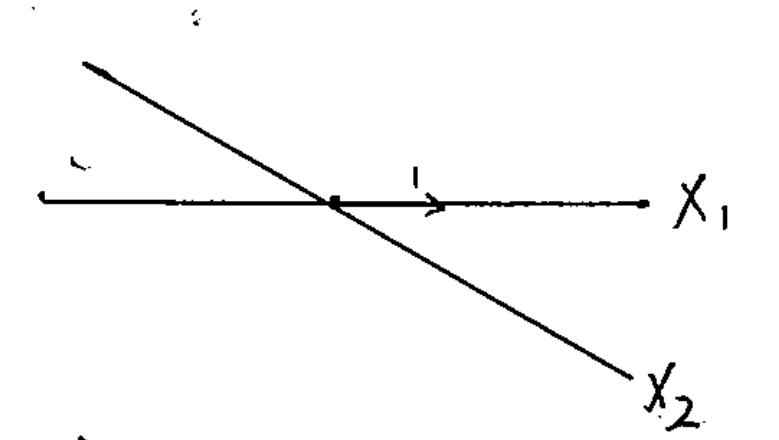
\includegraphics[width=2.1in,height=2.1in]{figures/ch05/figure1_a.jpg}
		%\caption{This is an inserted JPG graphic} 
		%\label{fig:graph} 
	\end{figure}
	$$ b) w = V^Tx = 
	\left[
	\begin{matrix}
	-\frac{1}{\sqrt{2}}\\
	\frac{1}{\sqrt{2}}
	\end{matrix}
	\right]
	$$
	\begin{figure}
		\centering
		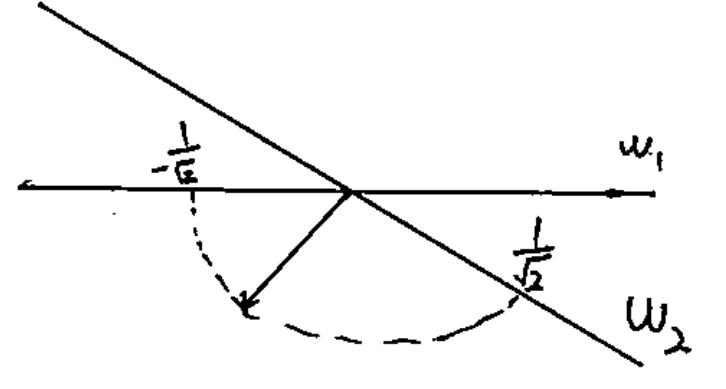
\includegraphics[width=2.1in,height=2.1in]{figures/ch05/figure1_b.jpg}
		%\caption{This is an inserted JPG graphic} 
		%\label{fig:graph} 
	\end{figure}
	$$ c) z = \Sigma w = 
	\left[
	\begin{matrix}
	-\frac{1}{\sqrt{2}}\\
	0\\
	0
	\end{matrix}
	\right]
	$$
	\begin{figure}
		\centering
		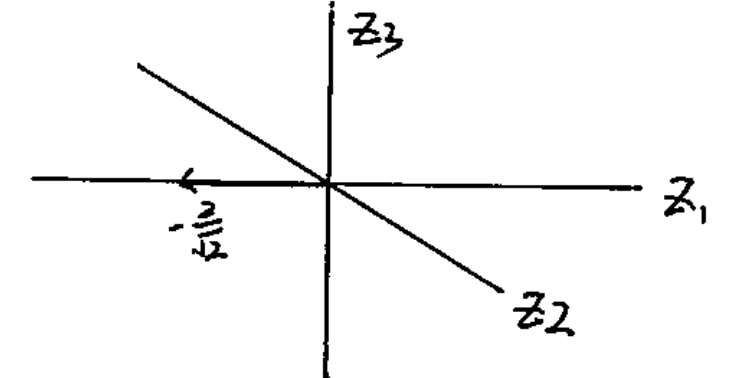
\includegraphics[width=2.1in,height=2.1in]{figures/ch05/figure1_c.jpg}
		%\caption{This is an inserted JPG graphic} 
		%\label{fig:graph} 
	\end{figure}
	$$ d) y = Uz =  
	\left[
	\begin{matrix}
	-\frac{2}{\sqrt{6}}\\
	-\frac{2}{\sqrt{6}}\\
	-\frac{2}{\sqrt{6}}
	\end{matrix}
	\right]
	$$
	\begin{figure}
		\centering
		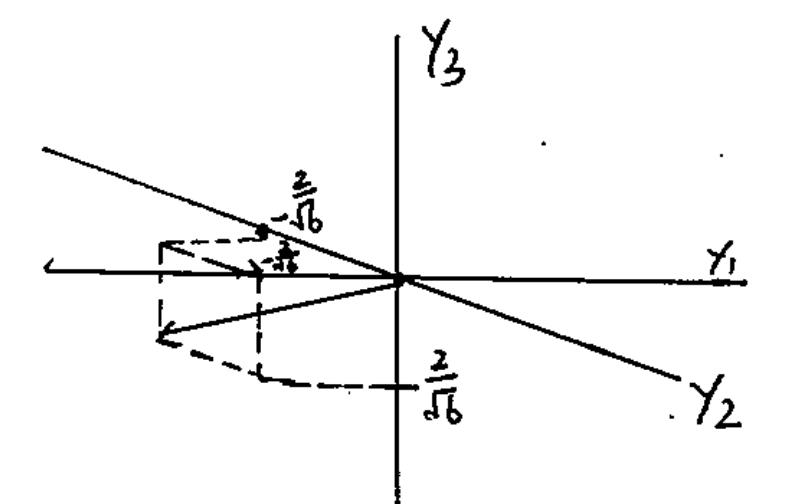
\includegraphics[width=2.1in,height=2.1in]{figures/ch05/figure1_d.jpg}
		%\caption{This is an inserted JPG graphic} 
		%\label{fig:graph} 
	\end{figure}
	
	
\end{example}


SVD follows from eigen-decomp of $A^TA$ and $AA^T$ $\rightarrow$ both symmetric, so spectral theorem applies. 

Write out $U\& V$ as: (r: rank($A$))



$$ U =   
\left[
\begin{matrix}
U^{(1)} & ... & U^{(r)} & U^{(r+1)} & ... & U^{(m)}
\end{matrix}
\right] =
\left[
\begin{matrix}
U_r & U_{mr}
\end{matrix}
\right]
$$


$$ V =   
\left[
\begin{matrix}
V^{(1)} & ... & V^{(r)} & V^{(r+1)} & ... & V^{(n)}
\end{matrix}
\right] =
\left[
\begin{matrix}
V_r & V_{nr}
\end{matrix}
\right]
$$




\begin{align*}
AA^T &= U\tilde{\Sigma} V^TV\tilde{\Sigma}^TU^T
&=
\begin{bmatrix}
\mathcal{U}_r & \mathcal{U}_{mr}
\end{bmatrix}
\begin{bmatrix}
\Sigma & \textbf{0}\\
\textbf{0}&\textbf{0}
\end{bmatrix}
\begin{bmatrix}
\Sigma^r & \textbf{0}\\
\textbf{0}&\textbf{0}
\end{bmatrix}
\begin{bmatrix}
\mathcal{U}_r^T\\
\mathcal{U}_{mr}^T
\end{bmatrix}
&=
\begin{bmatrix}
\mathcal{U}_r & \mathcal{U}_{mr}
\end{bmatrix}
\begin{bmatrix}
\Sigma^2 & \textbf{0}\\
\textbf{0}&\textbf{0}
\end{bmatrix}
\begin{bmatrix}
\mathcal{U}_r^T\\
\mathcal{U}_{mr}^T
\end{bmatrix}
&= \sum^r_{i=1}(\sigma_i)^2u^{(i)}(u&{(i)})^T\\
&= \sum^m_{i=1}(\sigma_1)^2u^{(i)}u^{(i)^T}
\end{align*}



$(AA^T)u^{(k)}$, $\rightarrow$ WTS $u^{(k)}$ is $k^{th}$ eigenvector of $AA^T$. 

$(AA^T)u^{(k)} = \sum^m_{i=1}\sigma_i^2u^{(1)}(u^{(1)})^Tu^{(k)} = \sum^n_{i=1}\sigma_i^2\prod(i=k)u^{(1)} =\sigma^2_ku^{(k)}$

$\lambda_k(AA^T) = \sigma^2_k$

same logic applied to $A^TA$ shows $V^{(k)}$ is $k^{th}$ eigenvector of $(A^TA)$


\subsection{Computing SVD}

1) Singular values: Compute eigenvalues of $AA^T$ or $A^TA$ to find $\lambda_i(A^TA) =\sigma_i^2$ $\rightarrow$ $\sigma_i = \sqrt{\lambda_i(A^TA)}$

$x^TA^TAx = w^Tw =||w||^2$

2) Right-Singular vectors: eigenvectors of $A^TA$;

3) Left-Singular vectors: eigenvectors of $AA^T$;

4) Because $AA^T \& A^TA$ both symmetric, both have full set of eigenvectors.\\

2. Consider arbitrary $x\in \Re^n$, 

\begin{align*}
Ax &= U\tilde{\Sigma} V^Tx\\
&= 
\begin{bmatrix}%
U_r & U_{mr}
\end{bmatrix}
\begin{bmatrix}%
\Sigma & \textbf{0}\\
\textbf{0}& \textbf{0}
\end{bmatrix}
\begin{bmatrix}%
V_r^T\\
V_{mr}^T
\end{bmatrix}x\\
&= 
\begin{bmatrix}%
U_r & U_{mr}
\end{bmatrix}
\begin{bmatrix}%
\Sigma\\
\textbf{0}
\end{bmatrix}
\begin{bmatrix}%
V_r^T
\end{bmatrix}x\\
&= \Sigma^r_{i=1}\sigma_iu^{(i)}(V^{(1)})^Tx (***)
\end{align*}
\\

Eq(*) looses all components of $x$ along $V^{(i)}$ directions when $r+1 \leq i \leq n$:

$\rightarrow$ i.e. columns of $V_{nr}$

$\rightarrow$ columns of $V_{nr}$ provide basis for $N(A)$.\\


All direction in output are in span $\{u^{(1)} ,..., u^{(n)}\}$

$\rightarrow$ columns of $U_r$ provide basis for $R(A)$.\\

Columns of $U_{mr}$ provide basis for $N(A^T)$\\

Columns of $V_{r}$ provide basis for $R(A^T)$


2) Consider arbitrary $x\in \Re^n$

\begin{align*}
A &= \mathcal{U}\tilde{\Sigma}V^r\\
&= 
\begin{bmatrix}
\mathcal{U}_r & \mathcal{U}_{mr}
\end{bmatrix}
\begin{bmatrix}
\Sigma & \mathbf{0}\\
\mathbf{0} & \mathbf{0}
\end{bmatrix}
\begin{bmatrix}
V_r^T\\
V_{nr}^T
\end{bmatrix}\\
&= 
\begin{bmatrix}
\mathcal{U}_r & \mathcal{U}_{mr}
\end{bmatrix}
\begin{bmatrix}
\Sigma \\
\mathbf{0} & 
\end{bmatrix}
\begin{bmatrix}
V_r^T
\end{bmatrix}\\
&= \mathcal{U}_r\Sigma V_r^T\\
\mathcal{U}_r^TAV_r &= \mathcal{U}_r^T(\mathcal{U}_r\Sigma V_r^T)V_r = \Sigma = \mathcal{U}_r^TAV_r
\end{align*}


\begin{align}
A &= \mathcal{U}_r\Sigma V_r^T \\
&= \sum^r_{i=1}\mathcal{U}^{(i)}(V^{(i)})^T\sigma_i\\
&= \sigma_1\mathcal{U}^{(1)}V^{(1)^T}+ \sigma_2\mathcal{U}^{(2)}V^{(2)^T}
\end{align}

\begin{equation*}
\sigma_1\mathcal{U}V^{(1)^T} = 
\begin{bmatrix}
\sigma_1V_1^{(1)}\mathcal{U}^{(1)} & \sigma_1V_2^{(1)}\mathcal{U}^{(1)} & ... & \sigma_1V_n^{(1)}\mathcal{U}^{(1)}
\end{bmatrix}
\end{equation*}

Condition \#

Consider $Ax = b$ when $A$ is invertible, solve for $x$ as $x = A^{-1}b$. What if $b = b_r + e$? how much does solution change? 

Solution is $\hat{x} = A^{-1}b_T + A^{-1}e$

\begin{equation*}
\frac{||\frac{A^{-1}e||}{||A^{-1}b_T||}}{\frac{||e||}{||b||}} = \frac{||A^{-1}e||_2}{||e||_2} \frac{||b||_2}{||A^{-1}b||_2}
\end{equation*}

\begin{align*}
max_{e,b\neq 0} \, \frac{||A^{-1}e||}{||e||} \frac{||b||}{||A^{-1}b||} &= \left[max_{e\neq 0}\, \frac{||A^{-1}e}{||e||}\right]\left[max_{b\neq 0}\, \frac{||b||}{||A^{-1}b||}\right]\\
&= \frac{\sigma_{max}(A^{-1})}{\sigma_{min}(A^{-1}}\\
&= \frac{\frac{1}{\sigma_n}}{\frac{1}{\sigma_1}}\\
&= \frac{\sigma_1}{\sigma_n}\\
&= \frac{\sigma_{max}(A)}{\sigma_{min}(A)}
&= K(A)
\end{align*}

\begin{figure}
	\centering
	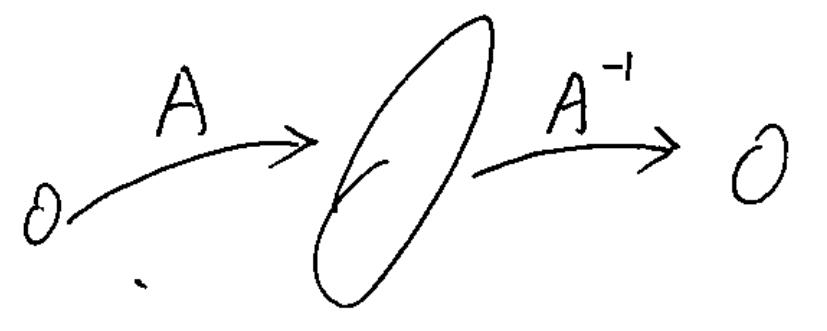
\includegraphics[width=2.1in,height=2.1in]{figures/ch05/figure2.jpg}
	%\caption{This is an inserted JPG graphic} 
	%\label{fig:graph} 
\end{figure}

\begin{align}
A^{-1} &= (\mathbb{U}\Sigma V^T)^{-1} \\
&= V\Sigma^{-1}\mathcal{T}\\
&= V
\begin{bmatrix}
\frac{1}{\sigma_1} & &\\
& ... & \\
& & \frac{1}{\sigma_n}
\end{bmatrix}
\mathcal{U}^T\\
\sigma_{max}(A^{-1}) = \frac{1}{\sigma_n}\\
\sigma_{min}(A^{-1}) = \frac{1}{\sigma_1}
\end{align}
